\title{Academic career planning using bayesian network}
\author{
        Ray Shulang Lei\\
	200253624\\ 
	Department of Computer Science\\
        University of Regina\\
        Regina, Saskatchewan, S4S0A2, Canada
}
\date{\today}

\documentclass[12pt]{article}
\setlength{\parindent}{0in}
\usepackage{graphicx}
\usepackage{parskip}

\begin{document}
\maketitle

\begin{abstract}
Most of the time, students going into universities without anticipating enough time/energy. Furthermore, they might set unrealistic graduation plans, thus risking their financial/career/relationship well-beings. Universities provide program advisers(experts) to help students, but human resources are too valuable in most situations. On the other hand, face to face consulting does not have good accessibility to students, thus the reason to seek for online automated solutions.
\end{abstract}



\section{Introduction}
Undergraduate programs often has prerequisite charts. These charts can be converted to decision trees. However, whether a student will graduated is usually affected by many uncertain factors. For example, some courses are only being offered under specific conditions; Some classes have great difficulties such that they can not be taken simultaneously; Some classes have lab time requirements thus increases students’ work load, and so on. Using Bayesian network seems to be well-suited for these uncertain situations.
Using node.js, Dlib C++ Library to build an web application that answers student queries about carrer planning questions.

\section{Course Prerequisite Inference}\label{Course Prerequisite Inference}
Here is a directed acrylic graph A to represent the course prerequisite relations.\\
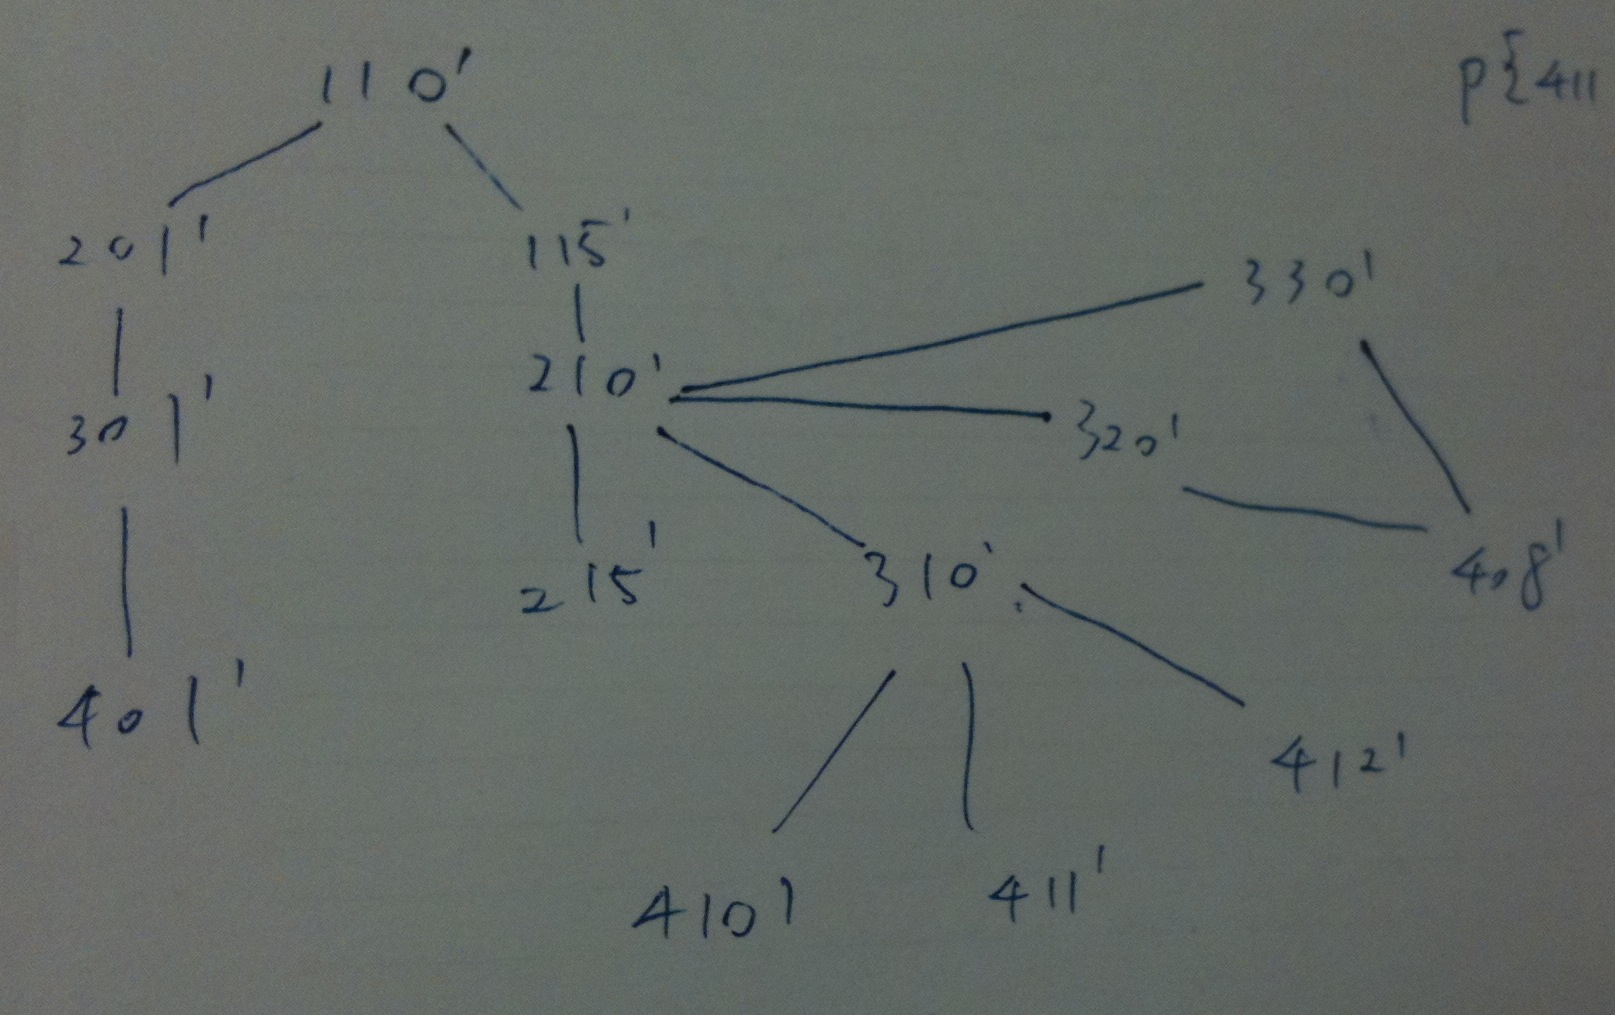
\includegraphics[scale=0.3]{g1_1.jpg}\\
Figure 1.1

i.e Querying the probability of taking CS411 in the future, provided student have taken CS110:\\
\begin{enumerate}
	\item Search the shortest path between $110'$ to $411'$ in A
	\item Which is $110' -> 115' -> 210' -> 310' -> 411'$
	\item The length of this path is 4, which means student needs at least 4 semesters to finish CS411, provided there is no class not bing offered during these semesters.
	\item If there are classes in the path not being offered, we need to add extra semesters accordingly.
	\item Run JTP on A, query $P\{CS411 = 1 \mid CS110 = 1\}$
	\item Provide feedback to student, telling the least semesters he need to finish CS411 with a probability.
\end{enumerate}

\section{Knowledge Aquisition}
I am working with Wendy Preikchat, who is the program coordinator at Computer Science Department. She has a lot of experience providing students consultations for their academic careers. There are also other people who helped with knowledge acquisitions: Ara Steininger, math department program coordinator; Shalini Mathias, Graduate Research Associate (curriculum design).


\section{Install, Run instructions}
Here are how to get the program running:
\begin{enumerate}
	\item git clone gzmask@lancewave.com:/home/gzmask/node\_bayes.git  (get the source code, password is '121212)
	\item go into node\_bayes folder
	\item run "sh server\_start.sh" to compile the source code. you'll need G++, make, node.js to compile.
	\item open browser, input the url: localhost:8080/index
	\item check your passed course, submit, then the bayesian network will tell you the possibilities that you would be able to pass the future classes
	\item executing "git pull" would update the source code to the newest version
\end{enumerate}
And ongoing and running instance can be directly  access at: http://142.3.31.224:8080/index    Open in Browser directly can avoice the trouble of compiling the source code and setting up the server yourself.

\section{Bayesian Network Implementation}
I used DLIB (http://dlib.net/) for the Bayesian Network part. The source code is hosted using GIT Repository, thus providing full advantage of easy to download and version management. The address of the GIT Repository is: gzmask@lancewave.com:/home/gzmask/nodebayes.git with password of '121212'.

Here is a simple explaination of the repository structure:
\begin{enumerate}
	\item README simple instruction on how to run the program
	\item app.js node.js starting point
	\item bayesnet.cpp bayesian network implementation
	\item bayesnet.h header file
	\item bayesianbind.cpp binding implementation between node.js and c++
	\item build binary files of the c++ compilation results
	\item dlib Dlib which provides data struture of Bayesian network and JTP
	\item doc this file
	\item examples 
	\item nodemodules node.js libraries
	\item oldbayesnet.cpp junk file
	\item package.json node.js package info metadata
	\item public html web file serving folder
	\item serverstart.sh shell script to execute the package
	\item views ejs html templates with node.js embeded code
	\item wscript c++ compilation linking information
\end{enumerate}

\section{User Interface}
The implementation of the User Interface is using the Node.js, which is based on the google chrome V8 engine. It provides fast javascript performance with good c++ interfacing abilities. At this point, the UI is still very simple.

\section{Results}\label{results}
The Node.js along side with C++ provides good performance and responsive web server.
A copy of source code is attached with this document.


\bibliographystyle{abbrv}
\bibliography{main}
\end{document}

